\section{Plant Analysis}
The linearized model is valid for an enough range of angles, so it can be used to do a deeper analysis on the behavior of the system. This includes evaluations in frequency domain, s-domain and L(s)-domain.

\subsection{Bode Diagram}
The Bode diagram gives the frequency response of the system, in both magnitude and phase plots, as seen in \figref{bodeTF}.\fxnote{redo picture, so that the phase label is not over the phase line in the figure}
\begin{figure}[H] 
	\centering 
	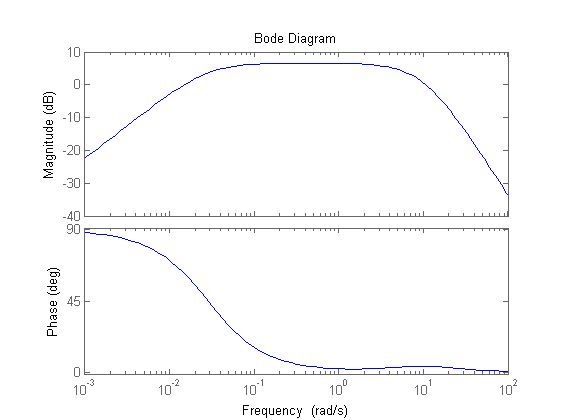
\includegraphics[scale=0.65]{figures/bodeTF}
	\caption{Bode diagram of the system}
	\label{bodeTF}
\end{figure} 

The graph also provides information about the stability of the system, given by the gain and phase margins. 

In this case the first one is just infinite because the phase never crosses \si{-180^o} and \si{180^o}.However, the phase margin is \si{-118^o}, which means that the phase has some margin before becoming unstable.

Looking only at the Bode plot, the system may be seen as stable, but the inverted pendulum is known to be an unstable system, so further analysis has to be done.

\subsection{Root Locus}
The Root Locus plot gives information about the location of the poles and zeros in open loop, and how the poles in closed loop will change as the gain of the whole system increases.

As seen in \figref{rlocusCubli} and \figref{rlocusCubliZoom} the system has one zero (s=0), and three poles (s=-10.6130, s=-0.0283 and s=9.3213). This means that the system is unstable as it has one pole in the right half plane (RHP) and, moreover, as one of the branches never crosses to the left half plane (LHP), the system can not be controlled just with a proportional controller.

\begin{minipage}{\linewidth}
	\begin{minipage}{0.53\linewidth}
		\begin{figure}[H]
			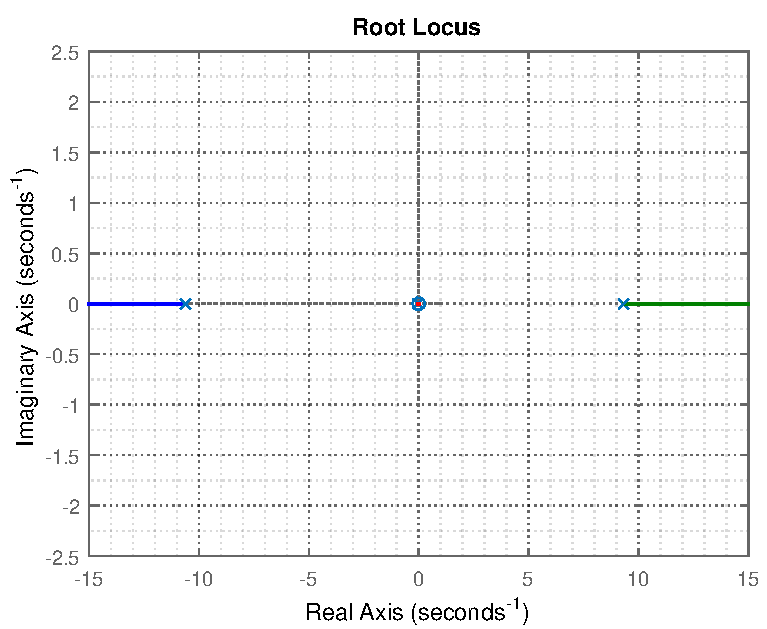
\includegraphics[scale=.4]{figures/rlocusCubli}
			\captionof{figure}{Root Locus of the system}
			\label{rlocusCubli}
		\end{figure}\vspace{-5mm}
	\end{minipage}
	\hspace{0.03\linewidth}
	\begin{minipage}{0.53\linewidth}
		\begin{figure}[H]
			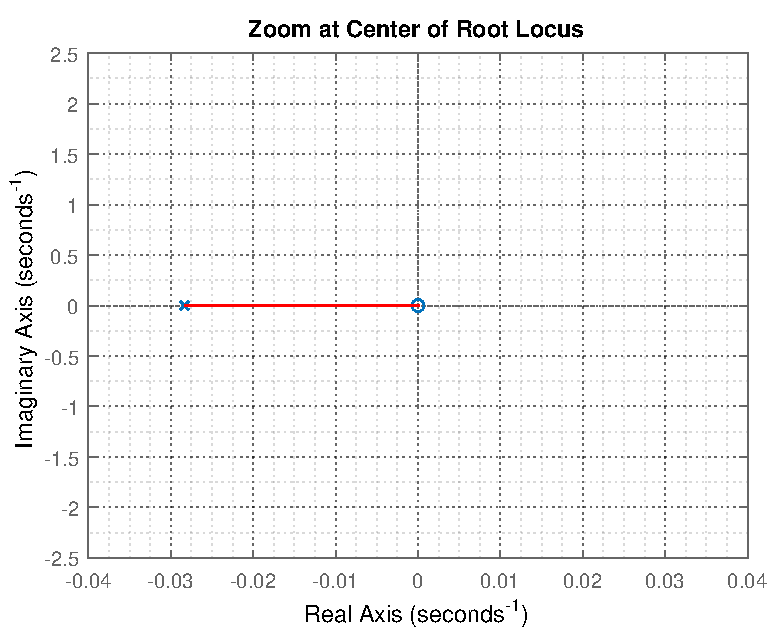
\includegraphics[scale=.4]{figures/rlocusCubliZoom}
			\captionof{figure}{Pole and zero next to the imaginary axis}
			\label{rlocusCubliZoom}
		\end{figure}\vspace{-5mm}
	\end{minipage}
\end{minipage}

\subsection{Nyquist Plot}
In any transfer function, the zeros of 1+L(s) (being L(s) the open loop function) become the poles of the closed loop system. That is why it is interesting to look at the Nyquist Stability Criterion, which can give information about this topic.

This criterion says that the number of zeros in the RHP of 1+L(s) (\si{Z_{RHP}}) is given by the number of poles of the OL (\si{P_{RHP}}) and the number of encirclements of the Nyquist plot around -1 (\si{N}).
\begin{flalign}
	\eq{Z_{RHP}}{N+P_{RHP}} 
	&\nonumber\\
	\label{FrameEq4OperatingPointZero}
\end{flalign}
In the case of this plant, the number of poles in the RHP is one and there are not circle surrounding -1 (\figref{nyquistCubli}), which means that the total number of zeros in the RHP is 1. As this zero will be a pole in the closed loop system the system is confirmed as unstable.

\begin{figure}[H] 
	\centering 
	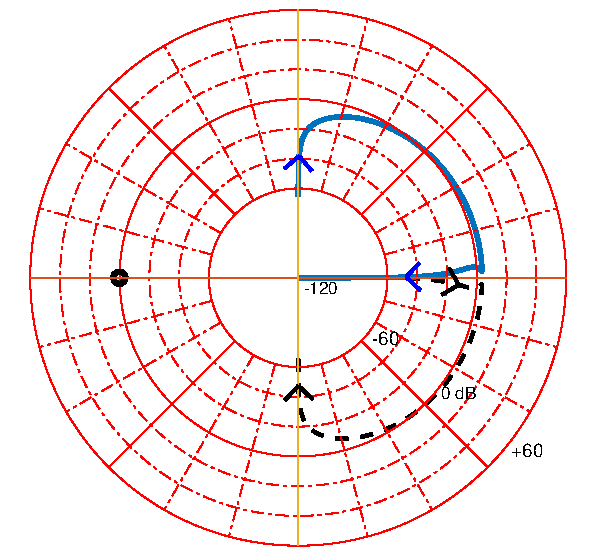
\includegraphics[scale=0.6]{figures/nyquistCubli}	
	\caption{Nyquist plot of the plant}
	\label{nyquistCubli}
\end{figure}
